\chapter*{Appendix}
\label{chapter:Appendix}
\pagestyle{Appendix}
\addcontentsline{toc}{chapter}{Appendix}

\section*{Appendix A: Programmcode}\label{Anh:programmcode}

\begin{lstlisting}[language=C, caption={\ac{pcm} \ac{udf} eicosane.c ohne Boussinesq-Approximation}, label={lst:udf_rest}]
//Modified UDF of the original source: https://akamcae.com/tutorials/phase-change-material-simulation-in-ansys-fluent/
#include "udf.h"
#include "mem.h"

//eicosane constant properties in solid phase
#define Ros_pcm 910.0
#define Cps_pcm 2132.4
#define Ks_pcm 0.4248

//eicosane constant properties in fluid phase
#define Rol_pcm 769.0
#define Cpl_pcm 2350.05
#define Kl_pcm 0.1505

//thermal expansion coefficient
#define TEC 0.0009

//solidus and liquidus temperatures of n-eicosane
#define Ts 309.0
#define Tl 311.0

//reference temperature for Boussinesq's approximation
#define Tr 310.0		//Fluent Tref must be equal to Tr

//density of PCM
DEFINE_PROPERTY(Ro_var_PCM,cell,thread)
{
	double Gama, Ro_pcm;
	#if !RP_HOST
		Gama=C_LIQF(cell,thread);
		Ro_pcm=(1-Gama)*Ros_pcm+Gama*Rol_pcm;
	#endif
	return Ro_pcm;
}

DEFINE_SPECIFIC_HEAT(Cp_var_PCM,T,Tref,h,yi)
{
	double Gama, Cp_pcm;
	#if !RP_HOST
		if (T<Ts) { Cp_pcm=Cps_pcm; } else if (T>=Ts&&T<=Tl)
		{
			Gama=(T-Ts)/(Tl-Ts);
			Cp_pcm=((1-Gama)*Ros_pcm*Cps_pcm+Gama*Rol_pcm*Cpl_pcm)/((1-Gama)*Ros_pcm+Gama*Rol_pcm);
		}
		else
		{
			Cp_pcm=Cpl_pcm;
		}
		*h=Cp_pcm*(T-Tref);
	#endif
	return Cp_pcm;
}

//thermal conductivity of eicosane
DEFINE_PROPERTY(K_var_PCM,cell,thread)
{
	double Gama, K_pcm;
	#if !RP_HOST
		Gama=C_LIQF(cell,thread);
		K_pcm=(1-Gama)*Ks_pcm+Gama*Kl_pcm;
	#endif
	return K_pcm;
}

//dynamic viscosity of PCM with fit
DEFINE_PROPERTY(Mu_var_PCM,cell,thread)
{
	double Temp,Mu_pcm;
	#if !RP_HOST
		Temp=C_T(cell,thread);
		Mu_pcm=(9*pow(10.,-4)*pow(Temp,2)-0.6529*Temp+119.94)*pow(10.,-3);
	#endif
	return Mu_pcm;
}

/*...*/
\end{lstlisting}

\section*{Appendix B: Simulationsergebnisse}\label{Anh:simulation}

\begin{figure}[H]
    \centering

    \begin{subfigure}{\textwidth}
        \centering
        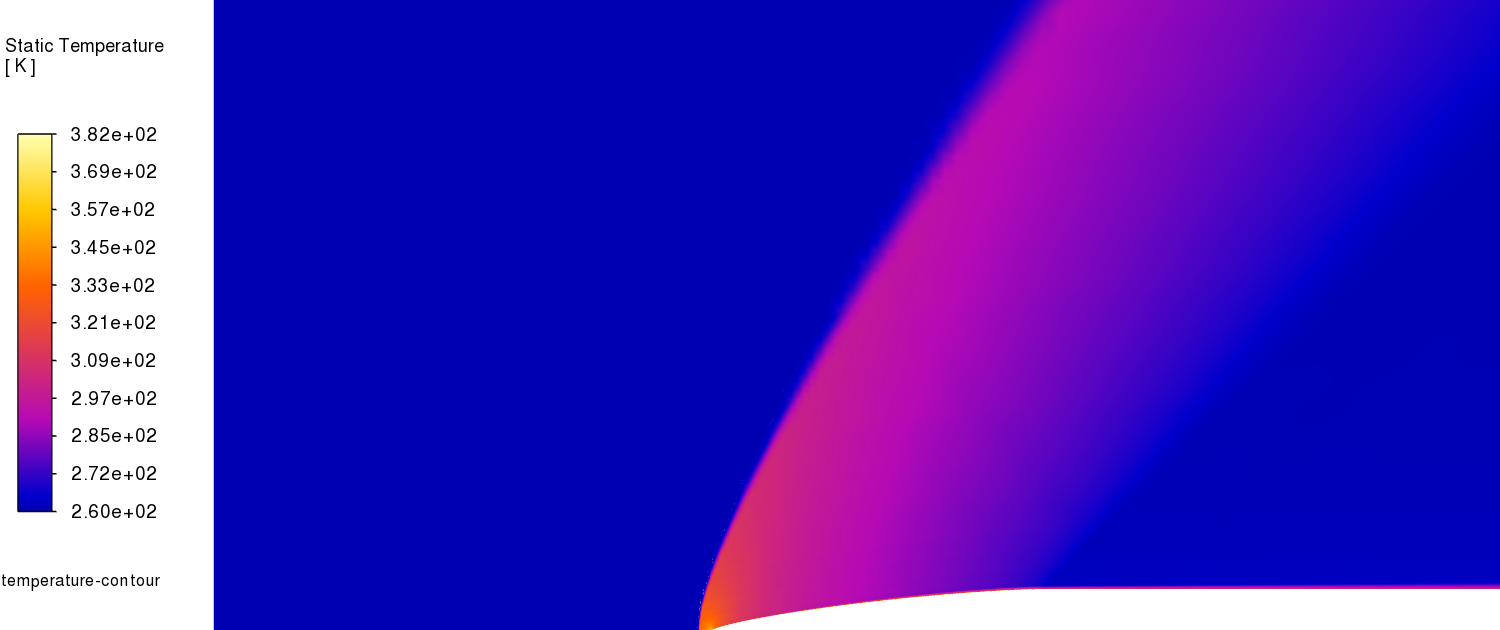
\includegraphics[height=0.23\textheight]{ansyspost/airflow/maxQminus10-temperature-contour.png}
        \caption{maxQ -\SI{10}{\second}}
        \label{fig:maxQminus10_temp_contour}
    \end{subfigure}

    \begin{subfigure}{\textwidth}
        \centering
        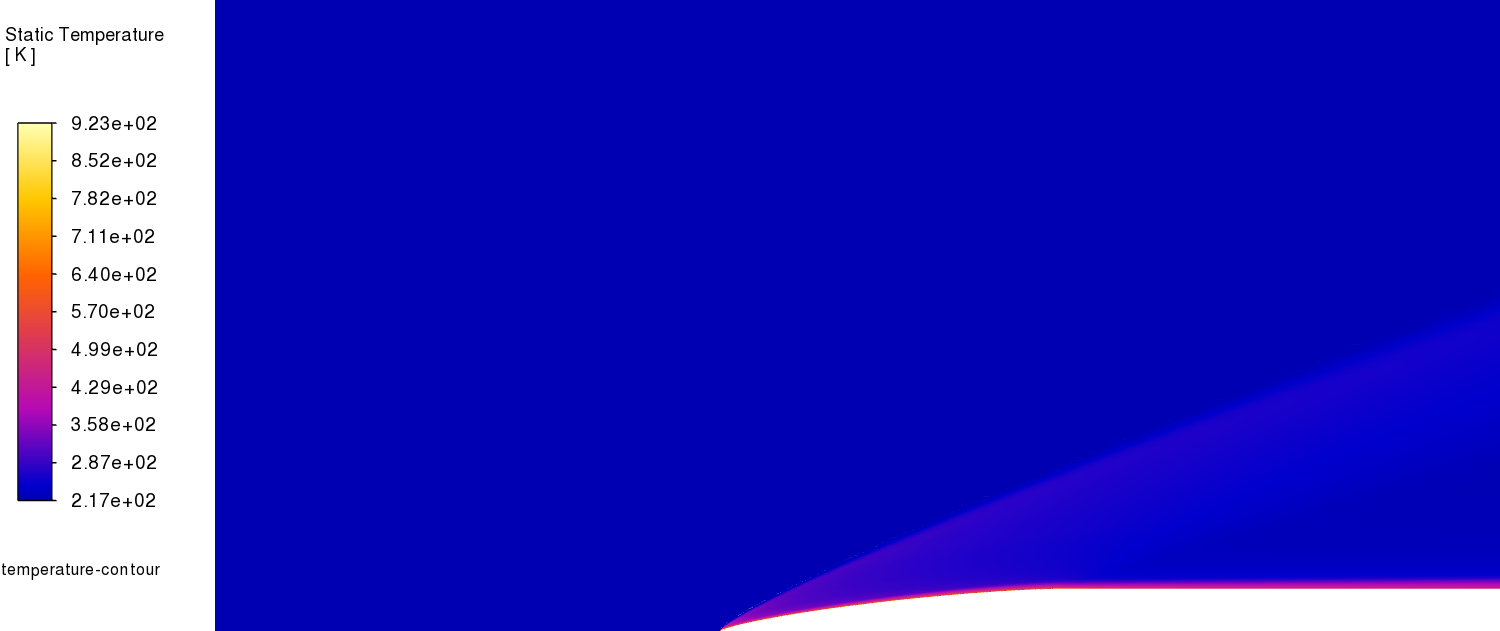
\includegraphics[height=0.23\textheight]{ansyspost/airflow/maxQplus10-temperature-contour.png}
        \caption{maxQ +\SI{10}{\second}}
        \label{fig:maxQplus10_temp_contour}
    \end{subfigure}

    \begin{subfigure}{\textwidth}
        \centering
        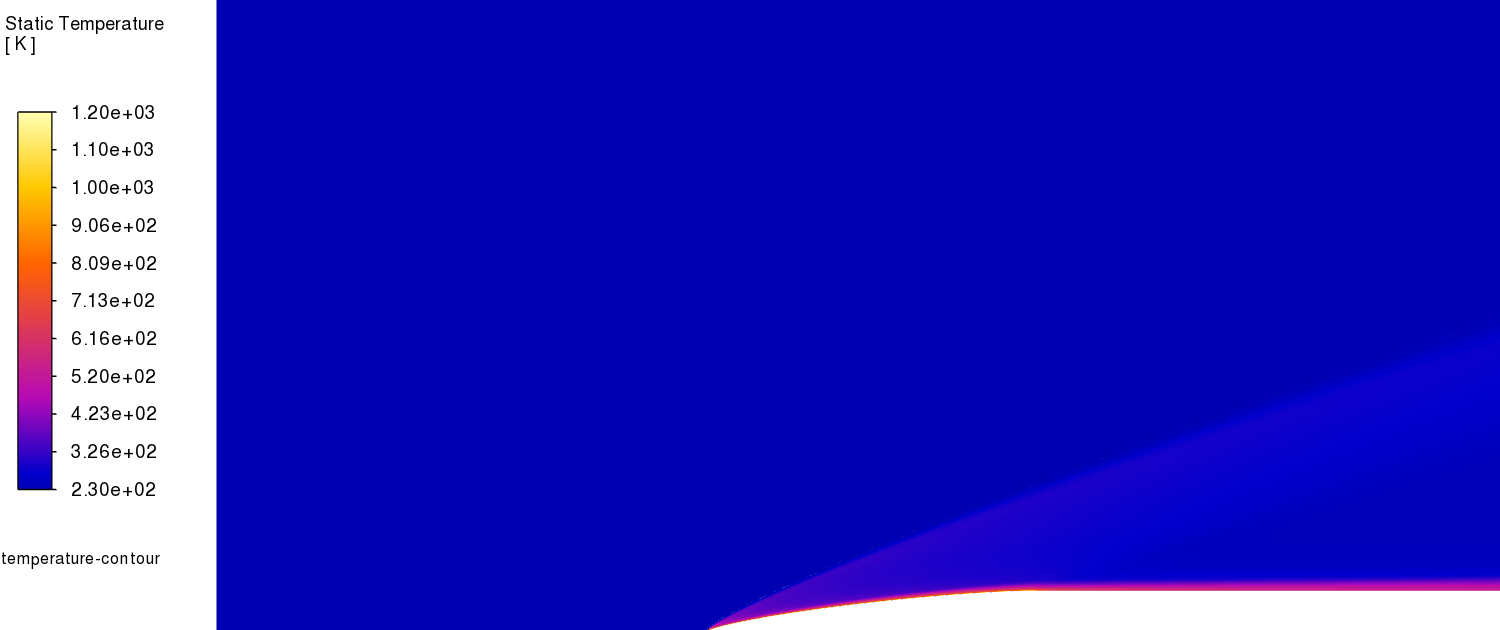
\includegraphics[height=0.23\textheight]{ansyspost/airflow/maxQplus20-temperature-contour.png}
        \caption{maxQ +\SI{20}{\second}}
        \label{fig:maxQplus20_temp_contour}
    \end{subfigure}

    \caption{Statische Temperaturkontur der Luft}
    \label{fig:airflow_temp_contour_continued}
\end{figure}

\begin{figure}[H]
    \centering

    \begin{subfigure}{\textwidth}
        \centering
        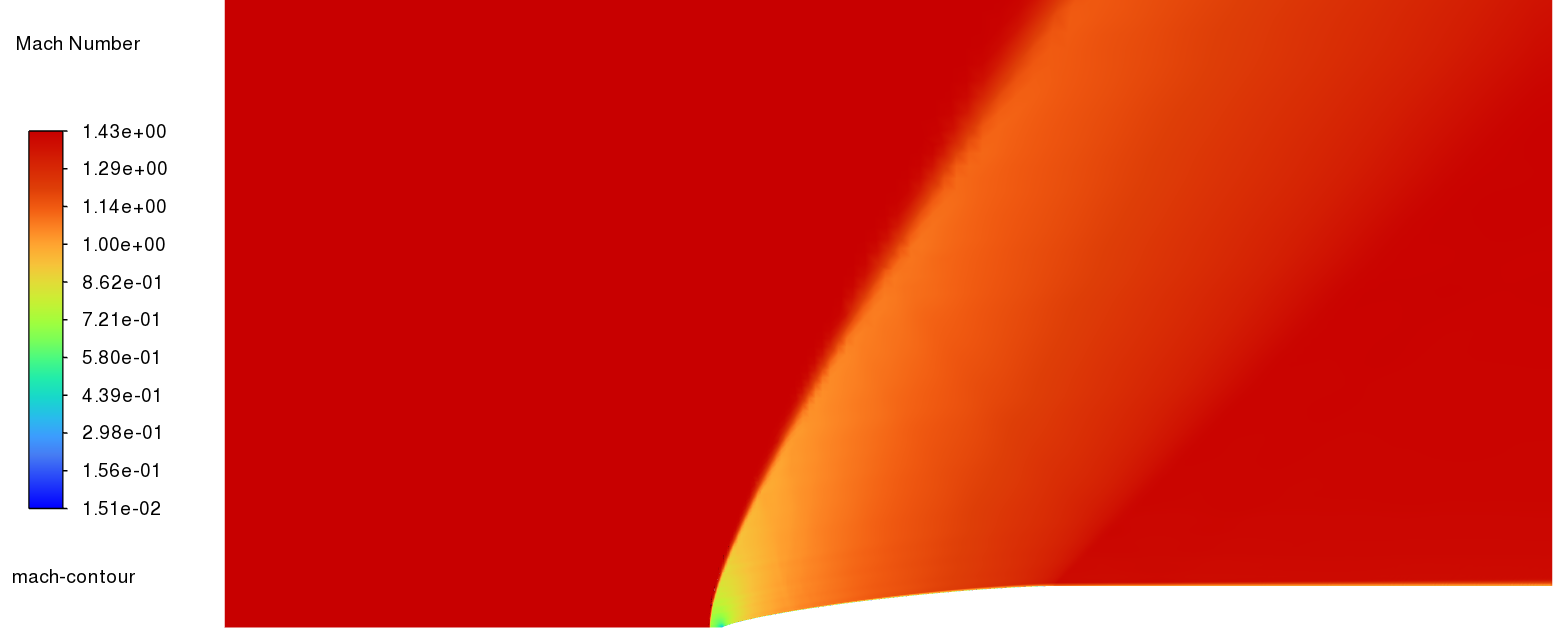
\includegraphics[height=0.23\textheight]{ansyspost/airflow/maxQminus10-mach-contour.png}
        \caption{maxQ -\SI{10}{\second}}
        \label{fig:maxQminus10_mach_contour}
    \end{subfigure}

    \begin{subfigure}{\textwidth}
        \centering
        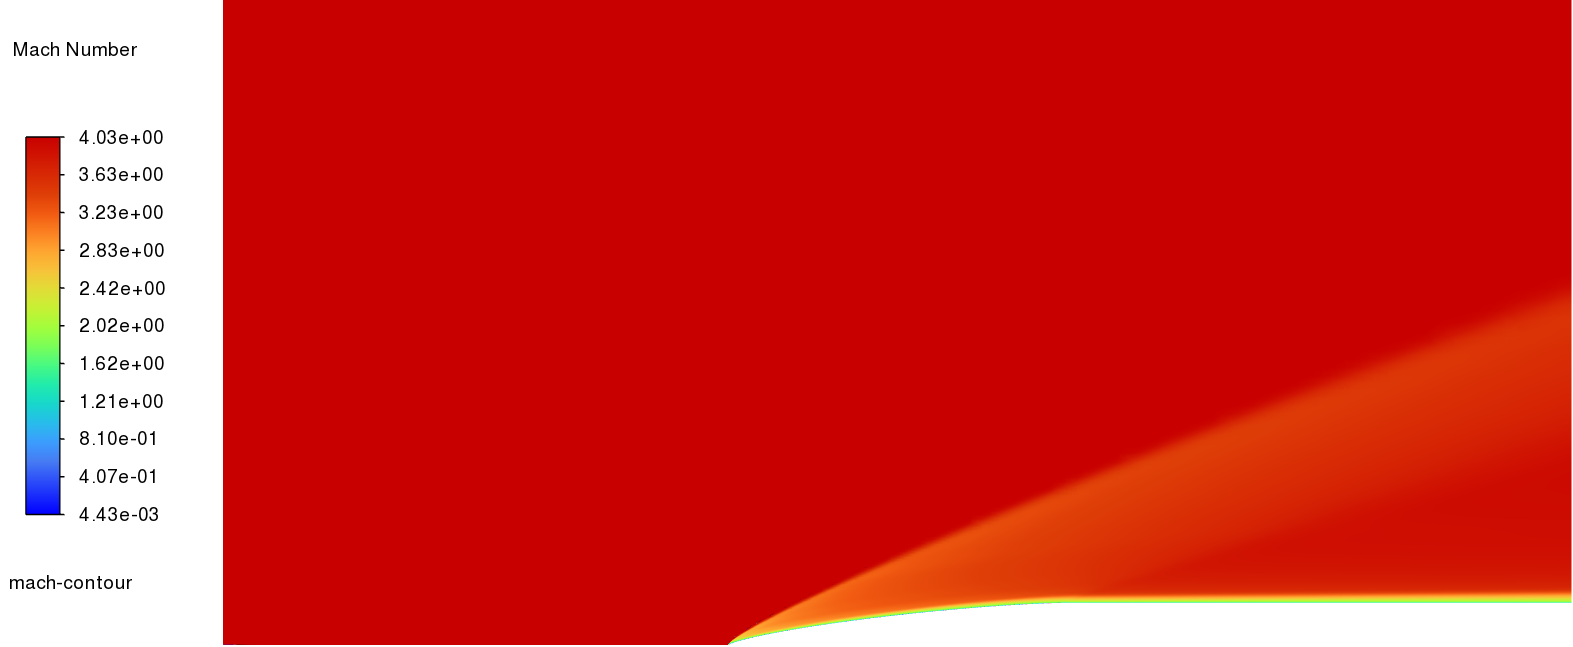
\includegraphics[height=0.23\textheight]{ansyspost/airflow/maxQplus10-mach-contour.png}
        \caption{maxQ +\SI{10}{\second}}
        \label{fig:maxQplus10_mach_contour}
    \end{subfigure}

    \begin{subfigure}{\textwidth}
        \centering
        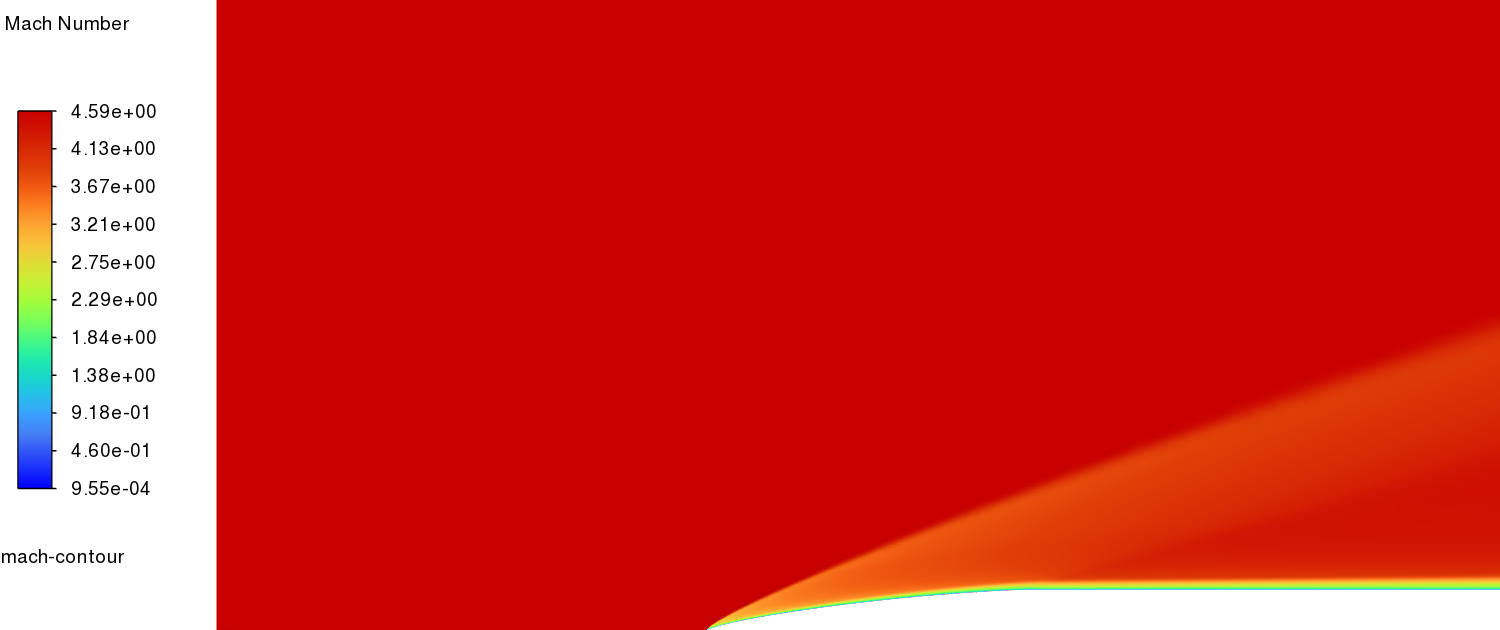
\includegraphics[height=0.23\textheight]{ansyspost/airflow/maxQplus20-mach-contour.png}
        \caption{maxQ +\SI{20}{\second}}
        \label{fig:maxQplus20_mach_contour}
    \end{subfigure}

    \caption{Machzahlkontur der Luft}
    \label{fig:airflow_mach_contour_continued}
\end{figure}

\begin{figure}[H]
    \centering

    \begin{subfigure}[t]{0.14\textwidth}
        \centering
        \raisebox{1\height}{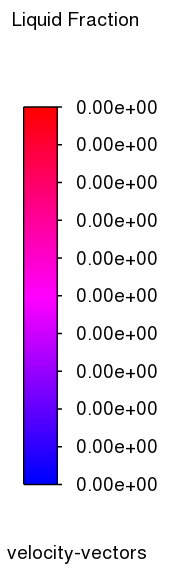
\includegraphics[height=0.2\textheight]{ansyspost/pcm/vector-legend.png}}
    \end{subfigure}%
    \hspace{2mm}% extra space between legend and first image
    \begin{subfigure}[t]{0.2\textwidth}
        \centering
        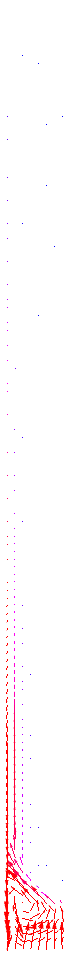
\includegraphics[height=0.7\textheight]{ansyspost/pcm/velocity-vector-300.png}
        \caption{\SI{300}{\second}}\label{fig:velocity_vector_300}
    \end{subfigure}%
    \begin{subfigure}[t]{0.2\textwidth}
        \centering
        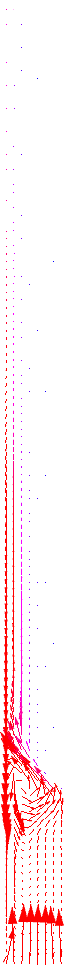
\includegraphics[height=0.7\textheight]{ansyspost/pcm/velocity-vector-600.png}
        \caption{\SI{600}{\second}}\label{fig:velocity_vector_600}
    \end{subfigure}%
    \begin{subfigure}[t]{0.2\textwidth}
        \centering
        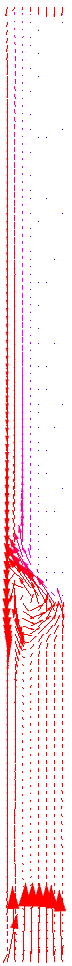
\includegraphics[height=0.7\textheight]{ansyspost/pcm/velocity-vector-900.png}
        \caption{\SI{900}{\second}}\label{fig:velocity_vector_900}
    \end{subfigure}%
    \begin{subfigure}[t]{0.2\textwidth}
        \centering
        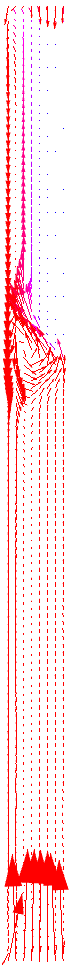
\includegraphics[height=0.7\textheight]{ansyspost/pcm/velocity-vector-1200.png}
        \caption{\SI{1200}{\second}}\label{fig:velocity_vector_1200}
    \end{subfigure}
    \caption{Konturen der statischen Temperatur. Die Legende bezieht sich auf~\ref{fig:temperatur_1200}}\label{fig:pcm_static_temperature_kontur}
\end{figure}